\chapter{Bounded principle curvatures}

Note that there sets in $\RR^3$ bounded by a closed surface $\Sigma$ with principle curvatures at most 1 by absolute value
that do not contain a ball of radius 1.

\begin{wrapfigure}{r}{33 mm}
\vskip-4mm
\centering
\includegraphics{mppics/pic-34}
\vskip0mm
\end{wrapfigure}

For example the region between two large spheres with similar radii and centers close to each other. 
This region can be made arbitrary thin and the curvature of the boundary can be made arbitrary close to zero.

The same example works in the plane --- a pair of circles with arbitrary small curvature can bound an arbitrary thin region.

\begin{thm}{Advanced exercise}
Suppose a set $V\subset \RR^3$ is bounded by a closed surface $\Sigma$ with principle curvatures bounded in absolute value by 1.
Assume that $V$ does not contain a ball of radius $\tfrac1{100}$.
Show that $\Sigma$ has two components of the same topological type; 
that is, both can be written in parametric form with the same parameter domain. 
\end{thm}


The same example would work for curves if we allow the boundary of the plane figure to be not connected.
The following question might look like a right 3-dimensional analog of the moon in a puddle problem (\ref{thm:moon}).

\section{Lagunov's example}

\begin{thm}{Question}
Assume a set $V\subset \RR^3$ is bounded by a closed connected surface $\Sigma$ with 
principle curvatures bounded in absolute value by 1.
Is it true that $V$ contains a ball of radius 1?
\end{thm}

It turns out that the answer is  ``no''. The following example was constructed by Vladimir Lagunov \cite{lagunov}.


\parit{Construction.}
Let us start with a body of revolution $V_1$ with cross section shown on the diagram.
The boundary curve of the cross section consists of 6 vertical line segments smoothly jointed into 3 closed simple curves. 
The boundary of $V_1$ has 3 components, each of which is a sphere.

\begin{figure}[h!]%{r}{43 mm}
%\vskip-4mm
\centering
\includegraphics{mppics/pic-33}
\vskip0mm
\end{figure}

A simple computation shows that if the curvature of all curves is at most 1 then the boundary surface of $V_1$ has priniple curvatures at most 1 in absolute value.

At most of the places $V_1$ can be made arbitrary thin,
the only thick place is where all tree spheres come together;
it could be arranged that the radius of the maximal ball is  just a little bit above 
\[r_2=\tfrac2{\sqrt{3}}-1< \tfrac16.\]
This is the radius of the smallest circle tangent to three unit circles that are tangent to each other.


It remains to modify $V_1$ to make its boundary connected without  alloing larger balls inside.

Note that each sphere in the boundary contains two flat discs;
they come into pairs close lying to each other. 
Let us drill thru two of such pairs and reconnect the holes by another body of revolution whose 
axis is shifted but stays parallel to the axis of $V_1$.
Denote the obtained body by $V_2$; its cross section of the obtained body is shown on the diagram. 

Then repeat the operation for the other two pairs.
Denote the obtained body by $V_3$; the cross section of the obtained body is shown on the diagram.

It is easy to see that the boundary of $V_3$ is connected
and assuming that the holes are large its boundary can be made so that its principle curvatures are still at most $1$.
\qeds

\begin{thm}{Claim}
The surface of $V_3$ has genus 2.
\end{thm}


\parit{Proof.}
Note that the boundary of $V_1$ consists of three spheres.

When we drill a hole, we make one hole in two spheres and two holes in one shpere.
We reconnect two spheres by a tube and obtain one sphere.
Connecting the two holes of the other sphere by a tube we get a torus.

At the second operation we make a torus from the remaining sphere and connect it to the other torus by a tube.
This way we get a sphere with two handles; that is, it has genus 2.
\qeds

\begin{thm}{Exercise}
Assume $V$ is a body of revolution in $\RR^3$ and its boundary is a connected surface with principle curvatures at most 1 in absolute value.
Show that $V$ contains a unit ball.
\end{thm}

\begin{thm}{Exercise}\label{ex:convex-lagunov}
Assume $V$ is a convex body in $\RR^3$ bounded by a surface with principle curvatures at most 1.
Show that $V$ contains a unit ball.%
\footnote{Hint: Consider a maximal ball in $V$ and apply Exercise~\ref{ex:projection} for a right choice of projection.}
\end{thm}





\begin{thm}{Exercise}
Modify Lagunov's construction to make the boundary surface a sphere with 4 handles.%
\footnote{Hint: Drill an extra hole or combine two examples together.}
\end{thm}



\begin{thm}{Advanced exercise}
Show that the bound in the Lagunov's example is optimal.
That is, if a body $V\subset \RR^3$ is bounded by a connected surface  $\Sigma$ with principle curvatures at most 1, then $V$ contains a ball of radius $r_2$.
\end{thm}

\section{On embedded sphere}


\begin{thm}{Advanced exercise}
Note that the body $V$ in the example of Lagunov is constructed by thikening a surface having a singular curve where the surface self-intersects at an angle of $120\degree$.
Show that this way one can not obtain a body bounded by a sphere.
\end{thm}

In fact one can show that if a body $V\subset \RR^3$ is bounded by a sphere $\Sigma$ with principle curvatures at most 1, then $V$ contains a ball of radius $r_3=\sqrt{\tfrac32}-1>\tfrac15$,
which is the radius of the smallest sphere tangent to three unit spheres that are tangent to each other.
Moreover, this bound is optimal.

An example of such a body can be obtained by thickening the so called Bing's house.
It is certainly a surface whose singularities are formed by three curves meeting at two points;
four ends at each point.
The remaining surface of Bing's house is smooth and has bounded principle curvatures;
we can assume that they are bounded by an arbitrary small number.

At the singular curves the three pieces of surface have to cross at angles $\tfrac23\cdot\pi$ and at the sigular points 6 pieces of surface should come together forming 6 tringles with vertex in the center of a regular tetrahedron and the bases at its 6 edges.
Thickening of a sufficiently large Bing's house of that type produces the optimal bound $r_3$ on the maximal ball that it contains.

\begin{wrapfigure}{o}{52 mm}
\vskip-0mm
\centering
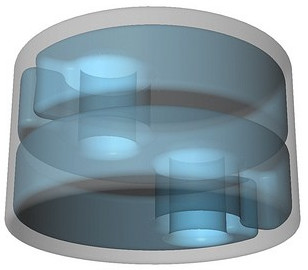
\includegraphics[scale=.45]{pics/thickened-bing's-house}
\vskip-0mm
\end{wrapfigure}

The thickening of Bing's house shown on the picture can not give the optimal bound,
but still it can produce an example of an embedded sphere that does not surround a ball of radius 1.

This picture is very similar to the Lagunov's example described above --- it can be obtained by filling the rings in the section of $V_3$ by thickened discs. 

This picture was taken from a post of Ken Baker \cite{baker};
this post has many other beautiful pictures that help to visualize Bing's house.

